\chapter{使用监督器实现容错}\label{chapt:fault-tolerent}

本章内容包括:
\begin{enumerate}
\item  如何使用 OTP Supervisor 行为
\item  学习如何使用 ETS,Erlang Term Storage
\item  如何将监督器与普通进程和其他 OTP 行为一起使用
\item  实现一个非常基础的 worker pool 应用
\end{enumerate}

在上一章中,我们使用语言提供的基本元素,即监视器、链接和进程,构建了一个简单的监督器。这应该让你对监督器的内部工作有了很好的理解。

在上一章中我们对你进行了一些挑逗,现在我们终于要使用真正的东西:\emph{OTP
Supervisor 行为}(以下简称为
Supervisor)。监督器的唯一责任是观察和检查一个附加的子进程是否崩溃,并在发生这种情况时采取一些行动。

OTP版本提供了比我们之前的实现更多的功能。例如,\emph{重启策略},它规定了如果出现问题,监督器应该如何重启子进程。
它还提供了在特定时间范围内限制重启次数的选项。这对于防止无限重启特别有用。

要\emph{真正}理解监督器,重要的是要亲自尝试一下。因此,我们将构建这个应用程序(由\emph{Observer}应用程序提供的全部展示):

\begin{figure}[!ht]
    \centering
    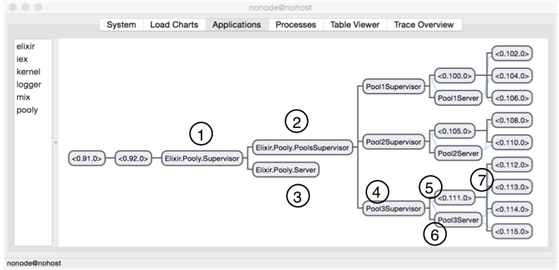
\includegraphics[width=0.8\linewidth]{6_1.png}
    \caption{完成的 worker pool 应用程序}
    \label{fig:6_1}
\end{figure}

图\ref{fig:6_1}显示了完成的 worker pool 应用程序。\#1 是顶级的\texttt{Supervisor}。
它监督 \#2,另一个\texttt{Supervisor}(\texttt{PoolsSupervisor}),
和一个\texttt{GenServer}(\texttt{Pooly.Server}),\#3。
\texttt{PoolsSupervisor}又监督了其他三个\texttt{PoolSupervisor}。
其中一个被标记为\#4。这些监督器都有唯一的名称。
每个\texttt{PoolSupervisor} 又监督了一个 worker supervisor\#5(由其进程 id 表示)和一个 GenServer \#6。
最后,\#7是实际的\texttt{Worker},他们将完成实际的工作。
如果你想知道\texttt{GenServer}是用来做什么的,它们主要是用来为``同一级别''的监督器维护状态。
例如,位于\#6 的 \texttt{GenServer} 帮助监督器 \#5 维护状态。

\section{实现 Pooly -- 一个 Worker Pool 应用}

我们将在两章的过程中构建一个 worker pool。你说什么是 worker
pool?它是管理一池(惊喜!)\texttt{Worker}的东西。你可能需要这个是为了管理对稀缺资源的访问。它可以是任何东西,从
Redis 连接池、web socket 连接池,甚至是 GenServer \texttt{Worker}池。

例如,如果你生成了一百万个进程,每个进程都需要连接到数据库。打开一百万个数据库连接是不切实际的。为了解决这个问题,创建了一个数据库连接池。每次进程需要数据库连接时,它会向池发出请求。一旦进程完成了数据库连接,它就会返回到池中。实际上,资源分配被委托给了
worker pool 应用。

我们将要构建的 worker pool 应用\emph{一点都不}简单。事实上,如果你熟悉
Poolboy,那么很多设计都是为了这个例子而改编的。如果你没有听说过或者没有使用过
Poolboy,也没关系,它不是先决条件。

我相信这是一个非常有益的练习,因为它让你思考那些在简单的例子中不会出现的概念和问题。
你也将亲手使用Supervisor API。

因此,这个例子可能比迄今为止的例子稍微有些挑战性。一些代码/设计可能不是很明显,但主要是因为你没有事后诸葛亮的好处。
但是不用担心,亲爱的读者,因为你将在每一步都得到指导。
我只要求你通过在电脑上输入代码来完成这个代码,然后在下一章的结束时期待启示。

\subsection{计划}

我们将通过四个版本来演进 Pooly 的设计。本章将介绍 Supervisor
的基础知识,并帮助你构建一个非常基础的版本(版本 1)的
Pooly。下一章将完全专注于构建 Pooly 的各种功能。

表\ref{tab:pooly-versions} 列出了 Pooly 的每个版本的特性:

\begin{longtable}[]{@{}ll@{}}
\toprule()
版本 & 特性 \\
\midrule()
\endhead
1 & 支持\emph{单个}池 \\
& 支持\emph{固定}数量的 worker \\
& 当消费者和/或 worker 进程失败时,不进行恢复 \\
2 & 与版本 1 相同 \\
& 当消费者和/或 worker 进程失败时,进行恢复 \\
3 & 支持\emph{多个}池 \\
& 支持\emph{可变}数量的 worker \\
4 & 与版本 3 相同 \\
& 允许 worker 溢出的可变大小的池 \\
& 当所有 worker 都忙时,为消费者进程排队 \\
\bottomrule()
\caption{Pooly 将在四个版本中经历的不同变化}
\label{tab:pooly-versions}
\end{longtable}


为了了解设计将如何演变,版本 1 和版本 2 的样子如下:

\begin{figure}[!ht]
    \centering
    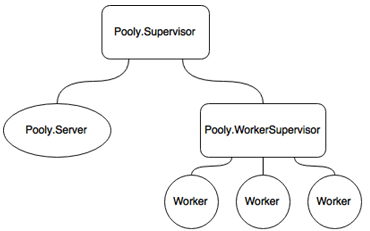
\includegraphics[width=0.8\linewidth]{6_2.png}
    \caption{Pooly 的版本 1 和版本 2}
    \label{fig:6_2}
\end{figure}

矩形代表 \texttt{Supervisor},椭圆代表\texttt{GenServer},圆圈代表 worker 进程。
在版本 3和版本 4 中,设计将如下所示演变:

\begin{figure}[!ht]
    \centering
    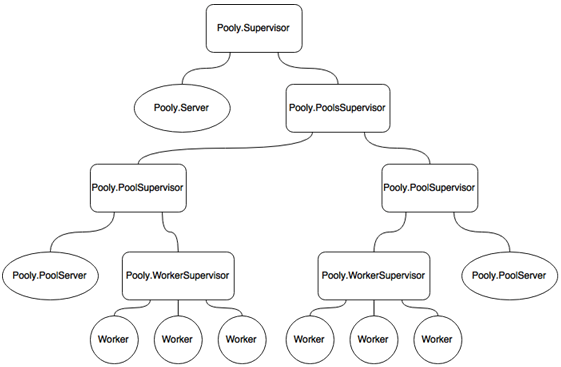
\includegraphics[width=0.8\linewidth]{6_3.png}
    \caption{Pooly 的版本 3 和版本 4}
    \label{fig:6_3}
\end{figure}

从图中,应该很明显为什么它被称为监督\emph{树}。

\subsection{Pooly 的样例运行}

在我们开始实际编码之前,看一下如何使用 Pooly 是很有指导意义的。这将涵盖
Pooly 的第一个版本。


\subsubsection{启动一个池}

为了启动一个池,必须给出一个\emph{池配置}。它提供了 Pooly
初始化池所需的信息。它看起来是这样的:

\begin{code}{}
\begin{minted}[linenos]{elixir}
pool_config = [
  mfa: {SampleWorker, :start_link, []},
  size: 5
]
\end{minted}
% \label{lst:id}
\end{code}

这告诉池创建五个\texttt{SampleWorker}。要启动池:

\begin{code}{}
\begin{minted}[linenos]{elixir}
Pooly.start_pool(pool_config)
\end{minted}
% \label{lst:id}
\end{code}


\subsubsection{检出 Workers}

在 Pooly 的术语中,\emph{检出} workers 意味着从池中请求并获取一个worker。
返回值是一个可用 worker 的 pid。

\begin{code}{}
\begin{minted}[linenos]{elixir}
worker_pid = Pooly.checkout()
\end{minted}
% \label{lst:id}
\end{code}

一旦\emph{消费者进程}获得了一个\texttt{worker\_pid},它可以随意使用它。
如果没有更多的worker 可用会发生什么?
目前,返回\texttt{:noproc}。
我们将在后续版本中提供更复杂的处理方式。


\subsubsection{将 Workers检入回池}

一旦消费者进程完成了 worker 的使用,它必须将其返回到池中,也称为检入worker。
检入 worker 是直接的:

\begin{code}{}
\begin{minted}[linenos]{elixir}
Pooly.checkin(worker_pid)
\end{minted}
% \label{lst:id}
\end{code}


\subsubsection{获取池的状态}

从池中获取一些有用的信息是很有用的。

\begin{code}{}
\begin{minted}[linenos]{elixir}
Pooly.status()
\end{minted}
% \label{lst:id}
\end{code}

目前,这返回一个元组,如\mintinline{elixir}|{3, 2}|。
这意味着有三个空闲的 worker和两个忙碌的 worker。
这就结束了 API 的简短介绍。

\subsection{深入 Pooly,版本 1:奠定基础}

转到你的目录,并使用 \texttt{mix}创建一个新项目:

\begin{code}{}
\begin{minted}[linenos]{elixir}
% mix new pooly
\end{minted}
% \label{lst:id}
\end{code}


\begin{note}{关于源代码的注意事项}
本章的这个项目的不同版本已经分成了不同的分支。
例如,要检出版本3,\texttt{cd} 进入项目文件夹,然后执行\texttt{git checkout version-3}。
\end{note}

\begin{note}{mix 和 --sup 选项}
你可能知道 \texttt{mix} 包含一个叫做\texttt{--sup} 的选项。
这个选项生成一个包含监督树的 OTP应用骨架。
如果省略了这个选项,应用将\emph{没有}监督器和应用回调生成。例如,你可能会想这样创建
Pooly:

\begin{code}{}
\begin{minted}[linenos]{elixir}
% mix new pooly --sup
\end{minted}
% \label{lst:id}
\end{code}

然而,由于我们正在学习,我们将选择无标志版本。
\end{note}

Pooly 的第一个版本只支持一个固定 worker 的单个池。
此外,当消费者或worker 进程失败时,不会进行恢复处理。
在这个版本结束时,Pooly将看起来像这样:

\begin{figure}[!ht]
    \centering
    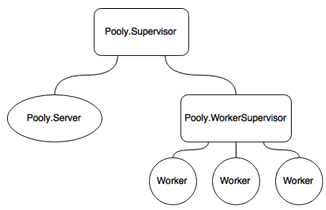
\includegraphics[width=0.8\linewidth]{6_4.png}
    \caption{Pooly 的版本 1}
    \label{fig:6_4}
\end{figure}


如你所见,应用程序由一个顶级监督器(\texttt{Pooly.Supervisor})组成,
它监督两个其他进程,一个GenServer 进程(\texttt{Pooly.Server})和一个 worker监督器(\texttt{Pooly.WorkerSupervisor})。
你可能会记得,从上一章开始,监督器可以自己被监督,因为监督器本身就是进程。

\begin{note}{我该如何开始?}
每当我设计可能有许多监督层次的 Elixir程序时,我总是先画一个草图。这是因为(你很快就会发现)你需要在脑海中保持相当多的东西。
可能比其他语言更多,你必须已经在脑海中有一个粗略的设计,这迫使你稍微提前思考。
\end{note}

当 Pooly 首次启动时,只有 \texttt{Pooly.Server} 附加到\texttt{Pooly.Supervisor}。
当使用池配置启动池时,\texttt{Pooly.Server}首先验证池配置是否有效。

之后,它向 \texttt{Pooly.Supervisor} 发送一个\texttt{:start\_worker\_supervisor}。
这个消息指示\texttt{Pooly.Supervisor} 启动\texttt{Pooly.WorkerSupervisor}。
最后,根据池配置中指定的\texttt{size},告诉\texttt{Pooly.WorkerSupervisor} 启动一定数量的 worker进程。

图\ref{fig:6_2a}说明了 Pooly 版本 1 的工作方式:

\begin{figure}[!ht]
    \centering
    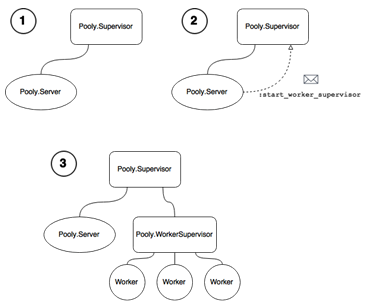
\includegraphics[width=0.8\linewidth]{6_2a.png}
    \caption{Pooly 的各个组件如何初始化}
    \label{fig:6_2a}
\end{figure}

\section{实现 Worker Supervisor}

我们首先将创建一个 worker supervisor。
这个 supervisor将负责监控池中生成的所有 worker。
在 \texttt{lib/pooly}中创建 \texttt{worker\_supervisor.ex}。
就像 GenServer行为(或者说\emph{任何}其他 OTP 行为),这就是如何使用 Supervisor 行为:

\begin{code}{}
\begin{minted}[linenos]{elixir}
defmodule Pooly.WorkerSupervisor do
  use Supervisor
end
\end{minted}
% \label{lst:id}
\end{code}

在代码\ref{lst:worker-supervisor}中,我们定义了老朋友 \texttt{start\_link/1}函数,它作为创建 supervisor 进程的主要入口点。
我们定义的\texttt{start\_link/1} 函数是一个包装函数,它调用\texttt{Supervisor.start\_link/2},并传入模块名和参数。

就像 GenServer 一样,当你定义\texttt{Supervisor.start\_link/2}时,你应该接着实现相应的 \texttt{init/1}回调函数。
传递给 \texttt{Supervisor.start\_link/2}的任何参数都会被传递给 \texttt{init/1} 回调。

\begin{code}{lib/pooly/worker\_supervisor.ex -- 使用模式匹配来验证和解构参数}
\begin{minted}[linenos]{elixir}
defmodule Pooly.WorkerSupervisor do
  use Supervisor

  #######
  # API #
  #######

  # 1
  def start_link({_, _, _} = mfa) do
    Supervisor.start_link(__MODULE__, mfa)
  end

  #############
  # Callbacks #
  #############

  # 2
  def init({m, f, a}) do
    # …
  end
end

# 1 模式匹配参数以确保参数确实是包含三个元素的元组。

# 2 从三元素元组中模式匹配各个元素。
\end{minted}
\label{lst:worker-supervisor}
\end{code}

在 \#1 中,我们声明 \texttt{start\_link}接受一个三元素元组,这将是 worker 进程的模块、函数和参数列表。

注意这里模式匹配的美妙之处。\texttt{\{\_,\_,\_\} = mfa}本质上做了\emph{两件}事。
首先,它断言输入参数必须是一个三元素元组。
其次,输入参数由\texttt{mfa} 引用。
我们可以把它写成\mintinline{elixir}|{m,f,a}|。
然而,由于我们没有使用单个元素,我们使用\texttt{mfa} 传递整个元组。

然后,\texttt{mfa} 被传递给\texttt{init/1}回调。
这次,我们需要使用元组的单个元素,因此在 \#2中我们断言预期的输入参数是\mintinline{elixir}|{m,f,a}|。
\texttt{init/1}回调是实际初始化发生的地方。

\subsection{初始化 Supervisor}

让我们仔细看看 \texttt{init/1} 回调,在 supervisor中,大部分有趣的部分都发生在这里:

\begin{code}{lib/pooly/worker\_supervisor.ex -- 使用子进程和 supervisor规范初始化 supervisor}
\begin{minted}[linenos]{elixir}
defmodule Pooly.WorkerSupervisor do
  #############
  # Callbacks #
  #############

  def init({m, f, a} = x) do
    worker_opts = [restart: :permanent, function: f]

    children = [worker(m, a, worker_opts)]

    opts = [strategy: :simple_one_for_one, max_restarts: 5, max_seconds: 5]

    supervise(children, opts)
  end
end
\end{minted}
\label{lst:worker-supervisor-init}
\end{code}

让我们学习如何解读代码\ref{lst:worker-supervisor-init}。
为了让 supervisor初始化其子进程,你必须给它一个\emph{子进程规范}。
子进程规范(我们在上一章简要介绍过)是supervisor 生成其子进程的配方。

子进程规范是用 \texttt{Supervisor.Spec.worker/3}创建的。
\texttt{Supervisor.Spec} 模块默认被 Supervisor行为导入,所以不需要提供完全限定的版本。

\texttt{init/1}回调的返回值必须是一个\emph{监督器规范}。
为了构造一个监督器规范,我们使用\texttt{Supervisor.Spec.supervise/2} 函数。

\texttt{supervise/2}接受两个参数。
第一个参数是\emph{子列表}。
第二个参数是\emph{选项的关键字列表}。
在上面的代码代码中,这分别由\texttt{children} 和 \texttt{opts}表示。

在我们定义子进程之前,让我们讨论一下\texttt{supervise/2} 的\emph{第二个}参数。

 \subsection{ 监督选项}

我们的示例将 \texttt{supervise/2} 的选项定义如下:

\begin{code}{}
\begin{minted}[linenos]{elixir}
opts = [strategy: :simple_one_for_one, max_restarts: 5, max_seconds: 5]
\end{minted}
% \label{lst:id}
\end{code}

这里可以设置一些选项。最重要的一个是\emph{重启策略},我们接下来会看到。

 \subsection{ 重启策略}

重启策略决定了当出现问题时,监督器如何重启子进程/子进程。为了定义重启策略,需要在重启策略中包含一个
\texttt{strategy} 键。有四种重启策略:

\begin{itemize}

\item
  \texttt{:one\_for\_one}
\item
  \texttt{:rest\_for\_one}
\item
  \texttt{:one\_for\_all}
\item
  \texttt{:simple\_one\_for\_one}
\end{itemize}

让我们快速看一下所有的策略。


\subsubsection{\texorpdfstring{\texttt{:one\_for\_one}}{:one\_for\_one}}

如果该进程死亡,只有该进程会被重启。所有其他进程都不受影响。


\subsubsection{\texorpdfstring{\texttt{:one\_for\_all}}{:one\_for\_all}}

就像三个火枪手一样,如果\emph{任何}进程死亡,监督树下的所有进程都会随之死亡。然后,所有的进程都会再次重启。如果监督树下的所有进程都相互依赖,这种策略就很有用。


\subsubsection{\texorpdfstring{\texttt{:rest\_for\_one}}{:rest\_for\_one}}

如果其中一个进程死亡,那么在该进程之后启动的其他进程都会被终止。然后,死亡的进程和剩余的子进程会被重启。可以把它想象成以圆形方式排列的多米诺骨牌。


\subsubsection{\texorpdfstring{\texttt{:simple\_one\_for\_one}}{:simple\_one\_for\_one}}

前三种策略用于构建静态监督树。这意味着,worker 是通过子进程规范预先指定的。

在 \texttt{:simple\_one\_for\_one}
中,你只需要在子进程规范中指定\emph{一个}条目。从这个监督器生成的每个子进程都会是\emph{同种}类型的进程。

理解 \texttt{:simple\_one\_for\_one}
策略的最好方式就像是一个工厂方法(或者说是 OOP
语言中的构造函数),其中``生产''的 worker
都是相似的。\texttt{:simple\_one\_for\_one}
用于我们想动态创建 worker 的情况。

监督器最初是以空 worker 开始的。然后,worker
动态地附加到监督器上。接下来,我们将看一下允许我们对监督器的行为进行微调的其他选项。


\subsection{最大重启次数和最大秒数}

\texttt{max\_restarts} 和
\texttt{max\_seconds}
转换为监督器在放弃并终止之前可以容忍的最大重启次数和最大秒数。

首先,为什么要有这样的东西呢?主要原因是你不希望你的监督器在真正出现问题时(程序员的错误?)无限制地重启其子进程。因此,你可能希望为监督器放弃的阈值指定一个值。注意,默认情况下,\texttt{max\_restarts}
和 \texttt{max\_seconds} 分别设置为 3 和 5。

在上面的代码代码中,我们指定如果在五秒内有超过五次重启,监督器应该放弃。

 \subsection{ 定义子进程}

现在是时候学习如何定义子进程了。在我们的代码中,子进程是在一个列表中指定的:

\begin{code}{}
\begin{minted}[linenos]{elixir}
children = [worker(m, a, worker_opts)]
\end{minted}
% \label{lst:id}
\end{code}

这告诉我们什么呢?它表示这个监督器有一个子进程,或者在
\texttt{:simple\_one\_for\_one}
重启策略的情况下,有一种\emph{类型}的子进程。(当我们通常不知道在使用
\texttt{:simple\_one\_for\_one} 重启策略时想生成多少个
worker 时,定义多个 worker 是没有意义的。)

\texttt{worker/3}
函数为\emph{worker}创建一个子进程规范,与其兄弟
\texttt{supervisor/3}
相反。这意味着,如果子进程\emph{不是}一个监督器,使用
\texttt{worker/3}。如果你正在监督一个监督器,那么使用
\texttt{supervise/3}。你很快就会使用这两种变体。

这两种变体都接受模块、参数和选项。前两个正如你所期望的那样。第三个参数更有趣。


\subsubsection{子进程规范默认选项}

默认情况下,当你像这样省略选项

\begin{code}{}
\begin{minted}[linenos]{elixir}
children = [worker(m, a)]
\end{minted}
% \label{lst:id}
\end{code}

Elixir 将提供以下选项作为默认值:

\begin{code}{}
\begin{minted}[linenos]{elixir}
[id: module, function: :start_link, restart: :permanent, shutdown: :infinity, modules: [module]]
\end{minted}
% \label{lst:id}
\end{code}


\subsubsection{function:Worker
的启动函数}

\texttt{function} 应该很明显 - 它是
\texttt{mfa} 的
\texttt{f}。有时,worker 的主要入口点是
\texttt{start\_link}
以外的其他函数。这是指定自定义函数要被调用的地方。

restart:重启值

我们将在整个 Pooly 应用中使用两个重启值:

· \texttt{:permanent} - 子进程总是被重启

· \texttt{:temporary} - 子进程永远不会被重启。

在 \texttt{worker\_opts} 中,我们指定了
\texttt{:permanent}。这意味着任何崩溃的 worker
总是会被重启。


\subsubsection{创建一个样例
Worker}

为了测试这个,我们需要一个样例 worker。在
\texttt{lib/pooly} 中创建
\texttt{sample\_worker.ex}。用以下内容填充它:

\begin{code}{lib/pooly/sample\_worker.ex -- 用于测试 Pooly 的 worker}

\begin{minted}[linenos]{elixir}
defmodule SampleWorker do
  use GenServer

  def start_link(_) do
    GenServer.start_link(__MODULE__, :ok, [])
  end

  def stop(pid) do
    GenServer.call(pid, :stop)
  end

  def handle_call(:stop, _from, state) do
    {:stop, :normal, :ok, state}
  end
end
\end{minted}
\label{lst:worker_to_test_supervisor}
\end{code}

\texttt{SampleWorker} 是一个非常简单的GenServer,除了有控制其生命周期的函数外,基本上什么都不做。

\begin{code}{}
\begin{minted}[linenos]{elixir}
iex > {:ok, worker_sup} = Pooly.WorkerSupervisor.start_link({SampleWorker, :start_link, []})
\end{minted}
% \label{lst:id}
\end{code}

现在,我们可以创建一个子进程:

\begin{code}{}
\begin{minted}[linenos]{elixir}
iex > Supervisor.start_child(worker_sup, [[]])
\end{minted}
% \label{lst:id}
\end{code}

返回值是一个看起来像 \mintinline{elixir}|{:ok, \#PID<0.132.0>}|
的两元素元组。向监督器添加更多的子进程。现在,让我们看一下 worker
supervisor 正在监督的所有子进程,使用
\texttt{Supervisor.which\_children/1}:

\begin{code}{}
\begin{minted}[linenos]{elixir}
iex > Supervisor.which_children(worker_sup)
\end{minted}
% \label{lst:id}
\end{code}

结果是一个看起来像这样的列表:

\begin{code}{}
\begin{minted}[linenos]{elixir}
[{:undefined, #PID<0.98.0>, :worker, [SampleWorker]},
{:undefined, #PID<0.101.0>, :worker, [SampleWorker]}]
\end{minted}
% \label{lst:id}
\end{code}

我们也可以计算子进程的数量:

\begin{code}{}
\begin{minted}[linenos]{elixir}
iex > Supervisor.count_children(worker_sup)
\end{minted}
% \label{lst:id}
\end{code}

返回结果应该是不言自明的:

\begin{code}{}
\begin{minted}[linenos]{elixir}
%{active: 2, specs: 1, supervisors: 0, workers: 2}
\end{minted}
% \label{lst:id}
\end{code}

现在来看看监督器的行动!创建另一个子进程,但这次,保存对它的引用:

\begin{code}{}
\begin{minted}[linenos]{elixir}
iex > {:ok, worker_pid} = Supervisor.start_child(worker_sup, [[]])
Supervisor.which_children(worker_sup)
\end{minted}
% \label{lst:id}
\end{code}

应该看起来像这样

\begin{code}{}
\begin{minted}[linenos]{elixir}
[{:undefined, #PID<0.98.0>, :worker, [SampleWorker]},
{:undefined, #PID<0.101.0>, :worker, [SampleWorker]},
{:undefined, #PID<0.103.0>, :worker, [SampleWorker]}]
\end{minted}
% \label{lst:id}
\end{code}

现在,让我们停止刚刚创建的 worker:

\begin{code}{}
\begin{minted}[linenos]{elixir}
iex > SampleWorker.stop(worker_pid)
\end{minted}
% \label{lst:id}
\end{code}

让我们检查一下 worker supervisor 的子进程的状态:

\begin{code}{}
\begin{minted}[linenos]{elixir}
iex(8)> Supervisor.which_children(worker_sup)
[{:undefined, #PID<0.98.0>, :worker, [SampleWorker]},
{:undefined, #PID<0.101.0>, :worker, [SampleWorker]},
{:undefined, #PID<0.107.0>, :worker, [SampleWorker]}]
\end{minted}
% \label{lst:id}
\end{code}

哇哦!监督器自动重启了停止的
worker!每当监督器自动重启失败的子进程时,我仍然会有一种温暖的感觉。在其他语言中获得类似的东西通常需要更多的工作。接下来,我们将看一下如何实现
\texttt{Pooly.Server}。

\section{实现服务器:操作的大脑}

现在,我们将处理操作的大脑。一般来说,你希望让监督器尽可能少的逻辑,因为代码越少,出错的可能性就越小。

因此,我们引入了一个 GenServer
进程,它将处理应用程序的大部分有趣的逻辑。服务器进程必须与顶级监督器和
worker 监督器进行通信。一种方法是使用\emph{命名进程}:

\begin{figure}[!ht]
    \centering
    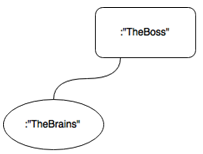
\includegraphics[width=0.8\linewidth]{6_3a.png}
    \caption{命名进程允许其他进程通过它们的名称引用它们}
    \label{fig:6_3a}
\end{figure}


在这种情况下,两个进程可以通过各自的名称相互引用。然而,更一般的解决方案是让服务器进程将对顶级监督器和worker 监督器的引用作为其\emph{状态}的一部分。

服务器将从哪里获得对两个监督器的引用呢?当顶级监督器启动服务器时,监督器可以将其自己的
pid 传递给服务器。事实上,这正是我们在实现顶级监督器时要做的事情。

\begin{figure}[!ht]
    \centering
    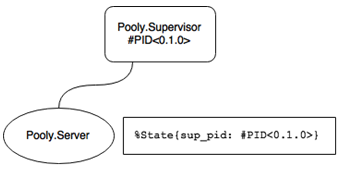
\includegraphics[width=0.8\linewidth]{6_3b.png}
    \caption{监督器的引用存储在 Pooly.Server 的状态中}
    \label{fig:6_3b}
\end{figure}


现在,由于服务器有了对顶级监督器的引用,它可以告诉它使用
\texttt{Pooly.WorkerSupervisor}
模块启动一个子进程,传入池配置的相关部分,然后
\texttt{Pooly.WorkerSupervisor} 将处理剩下的部分。

服务器进程还维护着池的状态。我们已经知道,服务器必须存储对顶级监督器和
worker
监督器的引用。它还应该存储什么呢?首先,它需要存储关于池的详细信息,比如要创建什么样的
worker,以及要创建多少个。池配置提供了这些信息。

 \subsection{ 池配置}

服务器接受一个以关键字列表形式的池配置。在这个版本中,一个示例池配置可能是这样的:

\begin{code}{}
\begin{minted}[linenos]{elixir}
[mfa: {SampleWorker, :start_link, []}, size: 5]
\end{minted}
% \label{lst:id}
\end{code}

键 \texttt{mfa} 代表要创建的 worker 池的
\texttt{m}odule(模块)、\texttt{f}unction(函数)和
\texttt{a}rguments(参数)列表。\texttt{size}
是要创建的 worker 进程的数量。

说了这么多,让我们看一些代码!创建一个名为\texttt{server.ex} 的文件,并将其放在\texttt{lib/pooly} 中。

目前,我们将使 \texttt{Pooly.Server}成为一个\emph{命名进程},
这意味着我们可以使用模块名(即\texttt{Pooly.Server.status} 而不是\texttt{Pool.Server.status(pid)})引用服务器进程。
代码\ref{lst:server-start-link} 展示了如何做到这一点:


\begin{code}{lib/pooly/server.ex --将对顶级监督器和池配置的引用传递给初始化服务器进程}

\begin{minted}[linenos]{elixir}
defmodule Pooly.Server do
  use GenServer
  import Supervisor.Spec

  #######
  # API #
  #######

  def start_link(sup, pool_config) do
    GenServer.start_link(__MODULE__, [sup, pool_config], name: __MODULE__)
  end
end
\end{minted}
\label{lst:server-start-link}
\end{code}

服务器进程需要对顶级监督器进程和池配置的引用,我们将其作为\texttt{[sup, pool\_config]} 传入。

现在,我们需要实现 \texttt{init/1}回调。
\texttt{init/1}回调有两个职责。
第一个是验证池配置。第二个是初始化状态,就像所有好的\texttt{init} 回调一样。

 \subsection{ 验证池配置}

有效的池配置看起来像这样:

\begin{code}{}
\begin{minted}[linenos]{elixir}
[mfa: {SampleWorker, :start_link, []}, size: 5]
\end{minted}
% \label{lst:id}
\end{code}

这是一个带有两个键 \texttt{mfa} 和\texttt{size}的关键字列表。任何其他键都将被忽略。
当函数遍历池配置关键字列表时,状态会逐渐建立起来:

\begin{code}{lib/pooly/server.ex -- 使用多个 init/2 函数子句设置服务器的状态}

\begin{minted}[linenos]{elixir}
defmodule Pooly.Server do
  use GenServer

  # 1
  defmodule State do
    defstruct sup: nil, size: nil, mfa: nil
  end

  #############
  # Callbacks #
  #############

  # 2
  def init([sup, pool_config]) when is_pid(sup) do
    init(pool_config, %State{sup: sup})
  end

  # 3
  def init([{:mfa, mfa} | rest], state) do
    init(rest, %{state | mfa: mfa})
  end

  # 4
  def init([{:size, size} | rest], state) do
    init(rest, %{state | size: size})
  end

  # 5
  def init([_ | rest], state) do
    init(rest, state)
  end

  # 6
  def init([], state) do
    # 7
    send(self, :start_worker_supervisor)
    {:ok, state}
  end
end
\end{minted}
% \label{lst:id}
\end{code}

代码 6.5 设置了服务器的状态。\#1 声明了一个
\texttt{struct},它作为服务器状态的容器。\#2 是当
\texttt{GenServer.start\_link/3} 被调用时的回调。

\texttt{init/1} 回调接收顶级监督器的 pid
和池配置。然后它调用
\texttt{init/2},它接收池配置和包含顶级监督器 pid
的新状态。

关键字列表中的每个元素都由一个两元素元组表示,其中第一个元素是键,第二个元素是值。

目前,我们对记住池配置的 \texttt{mfa} 和
\texttt{size} 值感兴趣。\#3 和 \#4
正是这样做的。如果我们想向状态添加更多字段,我们只需要添加更多具有适当模式的函数子句。\#5
忽略了我们不关心的任何选项。

最后,一旦我们像 \#6
那样遍历了整个列表,我们期望状态已经被初始化。记住,\texttt{init/1}
的有效返回值之一是 \mintinline{elixir}|{:ok, state}|。由于
\texttt{init/1} 调用
\texttt{init/2},并且在 \#6
中的空列表情况将是最后被调用的函数子句,因此它应该返回
\mintinline{elixir}|{:ok, state}|。

\#7 上的那行奇怪的代码是什么呢?一旦我们到达
\#6,我们就确信状态已经建立。这时我们可以启动我们之前实现的 worker
supervisor。发生的事情是,服务器进程向自己发送了一条消息。因为
\texttt{send/2} 立即返回,所以
\texttt{init/1} 回调不会被阻塞。你不希望
\texttt{init/1} 超时,对吧?

虽然 \texttt{init/1}
函数的数量可能看起来有些多,但不用担心。单独来看,每个函数都尽可能小。如果没有在函数参数中进行模式匹配,我们需要编写一个大的条件语句来捕获所有的可能性。


\subsection{启动 WorkerSupervisor}

当服务器进程使用 \texttt{send/2}向自己发送消息时,该消息将使用 \texttt{handle\_info/2}进行处理:

\begin{code}{lib/pooly/server.ex -- 启动 worker supervisor 的回调处理器}

\begin{minted}[linenos]{elixir}
defmodule Pooly.Server do
  defstruct sup: nil, worker_sup: nil, size: nil, workers: nil, mfa: nil

  #############
  # Callbacks #
  #############

  def handle_info(:start_worker_supervisor, state = %{sup: sup, mfa: mfa, size: size}) do
    # 1
    {:ok, worker_sup} = Supervisor.start_child(sup, supervisor_spec(mfa))
    # 2
    workers = prepopulate(size, worker_sup)
    # 3
    {:noreply, %{state | worker_sup: worker_sup, workers: workers}}
  end

  #####################
  # Private Functions #
  #####################

  defp supervisor_spec(mfa) do
    opts = [restart: :temporary]
    # 4
    supervisor(Pooly.WorkerSupervisor, [mfa], opts)
  end
end
\end{minted}
% \label{lst:id}
\end{code}

代码 6.6 中有很多事情正在进行。由于服务器进程的状态包含顶级监督器 pid(\texttt{sup}),我们使用监督器 pid 和监督器规范调用\texttt{Supervisor.start\_child/2}。
之后,我们传递新创建的worker 监督器 pid(\texttt{worker\_sup}),并使用它来启动\texttt{size} 数量的 worker。
最后,我们用 worker 监督器pid 和新创建的 worker 更新状态。

\#1 返回一个元组,其中 worker 监督器 pid 作为第二个元素。
在 \#4中,监督器规范由一个 worker监督器作为子进程组成。
注意,我们使用监督器变体,而不是

\begin{code}{}
\begin{minted}[linenos]{elixir}
worker(Pooly.WorkerSupervisor, [mfa], opts)
\end{minted}
% \label{lst:id}
\end{code}

我们使用监督器变体:

\begin{code}{}
\begin{minted}[linenos]{elixir}
supervisor(Pooly.WorkerSupervisor, [mfa], opts)
\end{minted}
% \label{lst:id}
\end{code}

这里,我们在 \#4 中作为监督器规范传入
\texttt{restart: :temporary}。这意味着顶级监督器不会自动重启
worker
监督器。这似乎有点奇怪。为什么呢?原因是我们想做的不仅仅是让监督器重启子进程。因为我们想要一些自定义的恢复规则,我们用
\texttt{restart: :temporary}
``关闭''了监督器自动重启失败的 worker 的默认行为。

请注意,这个版本并没有处理任何 worker
应该发生崩溃时的恢复。后续的版本将修复这个问题。接下来让我们处理 worker
的预填充。


\subsection{预填充 Worker Supervisor 的Worker}

给定池配置中的 \texttt{size} 选项,worker
监督器可以预填充自己的一组 worker。代码 6.7 中的
\texttt{prepopulate/2} 函数接收一个大小和 worker 监督器
pid,并构建一个 \texttt{size} 数量的 worker 列表,如
\#1 所示:

\begin{code}{lib/pooly/server.ex -- 预填充 worker supervisor 的 worker}

\begin{minted}[linenos]{elixir}
defmodule Pooly.Server do
  #####################
  # Private Functions #
  #####################

  defp prepopulate(size, sup) do
    prepopulate(size, sup, [])
  end

  defp prepopulate(size, _sup, workers) when size < 1 do
    workers
  end

  defp prepopulate(size, sup, workers) do
    # 1
    prepopulate(size - 1, sup, [new_worker(sup) | workers])
  end

  defp new_worker(sup) do
    # 2
    {:ok, worker} = Supervisor.start_child(sup, [[]])
    worker
  end
end

# 1 创建了一个附加到 worker 监督器的 worker 列表。 
# 2 动态创建一个worker 进程并将其附加到监督器。
\end{minted}
% \label{lst:id}
\end{code}




\subsection{创建新的 Worker进程}

代码 6.7 中的 \texttt{new\_worker/1}
函数值得一看。在这里,我们再次使用
\texttt{Supervisor.start\_child/2} 来生成 worker
进程。我们传入的是一个\emph{参数列表},而不是一个子进程规范。

Supervisor.start\_child/2 的两种形式

\texttt{Supervisor.start\\\_child/2}
有两种形式。第一种接受一个子进程规范:

\begin{code}{}
\begin{minted}[linenos]{elixir}
{:ok, sup} = Supervisor.start\_child(sup, supervisor\_spec(mfa))
\end{minted}
% \label{lst:id}
\end{code}

另一种形式接受一个参数列表:

\begin{code}{}
\begin{minted}[linenos]{elixir}
{:ok, worker} = Supervisor.start\_child(sup, [[]])
\end{minted}
% \label{lst:id}
\end{code}

你应该使用哪种形式呢?\texttt{Pooly.WorkerSupervisor}
使用的是 \texttt{:simple\\\_one\\\_for\\\_one}
重启策略。这意味着子进程规范已经被预定义了。这意味着第一种形式是不行的 -
你需要的是第二种形式。

第二种版本允许你向 worker 传递\emph{额外}的参数。在底层,当创建
\texttt{Pooly.WorkerSupervisor}
时在子进程规范中定义的参数会与传入
\texttt{Supevisor.start\\\_child/2}
的列表\emph{连接},然后结果会在初始化期间传递给 worker 进程。

\texttt{new\_worker/2} 的返回结果是新创建的 worker 的
pid。我们还没有实现从池中\emph{取出} worker,以及其对应的\emph{将 worker
放回}池中的方法。这两个操作也被分别称为\emph{取出}和\emph{归还}
worker。但在我们做这个之前,我们需要稍作改道,讨论一下下一节的 ETS。


\subsection{ETS初探}

在本章和下一章中,我们将使用 ETS,也称为 Erlang Term Storage。
本节将为你提供足够的背景知识,以理解本章和下一章中的 ETS相关代码。


\subsubsection{什么是 ETS}

它本质上是一个非常高效的内存数据库,专门用于存储 Erlang/Elixir
数据。它能够存储大量的数据而不会出现问题。数据访问也是在常数时间内完成的。它是
Erlang 的免费功能,这意味着我们必须使用 \texttt{:ets}
从 Elixir 中访问它。


\subsubsection{创建新的 ETS 表}

使用 \texttt{:ets.new/2}
创建表。让我们创建一个表来存储我妈妈最喜欢的艺术家,他们的出生日期和流派:

\begin{code}{}
\begin{minted}[linenos]{elixir}
iex > :ets.new(:mum_faves, [])
12308
\end{minted}
% \label{lst:id}
\end{code}

最基本的形式接受一个表示表名的原子和一个空的选项列表。\texttt{:ets.new/2}
的返回值是一个表 ID,类似于 pid。创建 ETS
表的进程被视为\emph{所有者进程}。在这种情况下,\texttt{iex}
进程是所有者。最常见的选项与 ETS
表的\emph{类型}、\emph{访问权限}以及是否\emph{命名}有关。


\subsubsection{ETS 表类型}

ETS 表有四种不同的形式:

\begin{itemize}

\item  \texttt{:set}

  \begin{itemize}
  
  \item
    这是默认的。它的特性与你在 CS101
    中可能学过的集合数据结构完全相同(无序,每个唯一键映射到一个元素)。
  \end{itemize}
\item  \texttt{:ordered\_set}

  \begin{itemize}
  
  \item    \texttt{:set} 的排序版本。
  \end{itemize}
\item  \texttt{:bag}

  \begin{itemize}
  
  \item    允许具有相同键的行,但行必须不同。
  \end{itemize}
\item  \texttt{:duplicate\_bag}

  \begin{itemize}
  
  \item    与 \texttt{:bag} 相同,但没有行唯一性的限制。
  \end{itemize}
\end{itemize}

在本章和下一章中,我们将使用\texttt{:set},这本质上意味着我们不需要在选项列表中指定表类型。
如果我们想要具体化,我们会这样创建表:

\begin{code}{}
\begin{minted}[linenos]{elixir}
iex > :ets.new(:mum_faves, [:set])
\end{minted}
% \label{lst:id}
\end{code}


\subsubsection{访问权限}

访问权限控制哪个进程可以从 ETS 表中读取和写入。有三个选项:

\begin{itemize}

\item  \texttt{:protected} -  所有者进程具有完全的读写权限。所有其他进程只能从中读取。这是默认设置。
\item  \texttt{:public} - 对读写没有限制。
\item  \texttt{:private} -  只有所有者进程可以从表中读取和写入。
\end{itemize}

在本章中,我们将使用 \texttt{:private}表,因为我们将存储其他池无权知道的与池相关的数据。
所以,假设我的妈妈对她的折衷音乐品味非常害羞,想要将表设为私有:

\begin{code}{}\begin{minted}[linenos]{elixir}
iex > :ets.new(:mum_faves, [:set, :private])
\end{minted}
% \label{lst:id}
\end{code}


\subsubsection{命名表}

注意,当我们创建 ETS
表时,我们提供了一个原子。这有些误导,因为我们\emph{不能}在不提供\texttt{:named\_table} 选项的情况下使用\texttt{:mum\_faves} 来引用表。
因此,要使用\texttt{:mum\_faves} 而不是像\texttt{12308} 这样的无法理解的引用,你可以这样做:

\begin{code}{}\begin{minted}[linenos]{elixir}
iex > :ets.new(:mum_faves, [:set, :private, :named_table])
\end{minted}
% \label{lst:id}
\end{code}

\texttt{:mum\_faves}
注意,如果你再次尝试运行上面的行,你会得到:

\begin{code}{}\begin{minted}[linenos]{elixir}
iex> :ets.new(:mum_faves, [:set, :private, :named_table])
** (ArgumentError) argument error
(stdlib) :ets.new(:mum_faves, [:set, :private, :named_table])
\end{minted}
% \label{lst:id}
\end{code}

这是因为名称应该是 ETS 表的\emph{唯一}引用。


\subsubsection{插入和删除数据}

使用 \texttt{:ets.insert/2}函数插入数据。
第一个参数是表标识符(数字或名称),第二个参数是数据。
数据以元组的形式出现,其中第一个元素是键,第二个可以是\emph{任何}、\emph{任意嵌套}的项。
这里有一些我妈妈的最爱:

\begin{code}{}\begin{minted}[linenos]{elixir}
iex > :ets.insert(:mum_faves, {"Michael Bolton", 1953, "Pop"})
true
iex > :ets.insert(:mum_faves, {"Engelbert Humperdinck", 1936, "Easy Listening"})
true
iex > :ets.insert(:mum_faves, {"Justin Beiber", 1994, "Teen"})
true
iex > :ets.insert(:mum_faves, {"Jim Reeves", 1923, "Country"})
true
iex > :ets.insert(:mum_faves, {"Cyndi Lauper", 1953, "Pop"})
true
\end{minted}
% \label{lst:id}
\end{code}

我们可以使用 \texttt{:ets.tab2list/1} 查看表中的内容:

\begin{code}{}\begin{minted}[linenos]{elixir}
iex > :ets.tab2list(:mum_faves)

[
  {"Michael Bolton", 1953, "Pop"},
  {"Cyndi Lauper", 1953, "Pop"},
  {"Justin Beiber", 1994, "Teen"},
  {"Engelbert Humperdinck", 1936, "Easy Listening"},
  {"Jim Reeves", 1923, "Country"}
]
\end{minted}
% \label{lst:id}
\end{code}

注意返回结果是一个列表,列表中的元素是无序的。好吧,我撒谎了。
我的妈妈其实并不是Justin Beiber的粉丝\pagenote{她也不是Cyndi Lauper 的粉丝,但我在写这篇文章的时候正在听 ``Girls just want to have fun''。}。
让我们纠正这一点:

\begin{code}{}\begin{minted}[linenos]{elixir}
iex > :ets.delete(:mum_faves, "Justin Beiber")
true
\end{minted}
% \label{lst:id}
\end{code}


\subsubsection{查找数据}
如果我们不能检索数据,那么表就没有用。最简单的方法是使用键。迈克尔·博尔顿的出生年份是什么?让我们找出来:

\begin{code}{}\begin{minted}[linenos]{elixir}
iex > :ets.lookup(:mum_faves, "Michael Bolton")
[{"Michael Bolton", 1953, "Pop"}]
\end{minted}
% \label{lst:id}
\end{code}

为什么结果是一个列表?回想一下,ETS 支持其他类型,比如\texttt{:duplicate\_bag},它允许重复的行。
因此,表示这个的最通用的数据结构就是简单的列表。

如果你想按\emph{年份}进行搜索怎么办?我们可以使用\texttt{:ets.match/2}:

\begin{code}{}\begin{minted}[linenos]{elixir}
iex > :ets.match(:mum_faves, {:"$1", 1953, :"$2"})
[["Michael Bolton", "Pop"], ["Cyndi Lauper", "Pop"]]
\end{minted}
% \label{lst:id}
\end{code}

我们传入一个\emph{模式},乍一看可能有点奇怪。
由于我们只是使用年份进行查询,我们使用\texttt{\$N} 作为占位符,其中\texttt{N}是一个整数。
这些数字对应于每个匹配结果中元素的顺序。让我们交换占位符:

\begin{code}{}
\begin{minted}[linenos]{elixir}
iex(20) > :ets.match(:mum_faves, {:"$2", 1953, :"$1"})
[["Pop", "Michael Bolton"], ["Pop", "Cyndi Lauper"]]
\end{minted}
% \label{lst:id}
\end{code}

你现在可以清楚地看到,流派在艺术家名字之前。如果你只关心返回艺术家呢?我们可以使用下划线来省略流派,就像这样:

\begin{code}{}
\begin{minted}[linenos]{elixir}
iex(25) > :ets.match(:mum_faves, {:"$1", 1953, :_})
[["Michael Bolton"], ["Cyndi Lauper"]]
\end{minted}
% \label{lst:id}
\end{code}

关于 ETS 还有更多的知识要学,但这就是你需要理解代码中 ETS部分的所有信息。
让我们回到从池中取出 worker 的问题。

 \subsection{ 检出 Worker}

当消费者进程从池中检出一个 worker时,有一些关键的物流问题需要处理,比如:

\begin{itemize}

\item  消费者进程的 pid 是什么?
\item  消费者进程正在使用哪个 worker pid?
\end{itemize}

服务器需要\emph{监控}消费者进程,因为如果它死掉,服务器进程需要知道并采取恢复行动。再次强调,我们还没有实现恢复代码,但正在打下基础。

我们还需要知道消费者进程使用的是哪个worker,这样我们就可以确定哪个消费者进程使用了哪个 workerpid。下面是检出 worker 的实现:

\begin{code}{lib/pooly/server.ex -- 检出 worker}

\begin{minted}[linenos]{elixir}
defmodule Pooly.Server do
  #######
  # API #
  #######

  def checkout do
    GenServer.call(__MODULE__, :checkout)
  end

  #############
  # Callbacks #
  #############

  # 1
  def handle_call(:checkout, {from_pid, _ref}, %{workers: workers, monitors: monitors} = state) do
    # 2
    case workers do
      [worker | rest] ->
        # 3
        ref = Process.monitor(from_pid)
        # 4
        true = :ets.insert(monitors, {worker, ref})
        {:reply, worker, %{state | workers: rest}}

      [] ->
        {:reply, :noproc, state}
    end
  end
end
\end{minted}
% \label{lst:id}
\end{code}

我们将使用 ETS表来存储监视器。
回调函数的实现很有趣。有两种情况需要处理。
要么我们还有剩余的worker 可以检出,要么我们没有。
在后一种情况下,我们返回\mintinline{elixir}|{:reply, :noproc, state}|,表示没有可用的进程。
在大多数关于GenServers 的例子中,你会看到 \texttt{from}参数通常被忽略:

\begin{code}{}
\begin{minted}[linenos]{elixir}
def handle_call(:checkout, _from, state) do
  # …
end
\end{minted}
% \label{lst:id}
\end{code}

在这种情况下,\texttt{from}是\emph{非常}有用的。
注意,\texttt{from}实际上是一个由客户端 pid 和标签(引用)组成的两元素元组。
在 \#1中,我们只关心客户端的 pid。
我们使用客户端的 pid(\texttt{from\_pid}) 并让服务器进程监控它。
然后在 \#4中我们使用生成的引用并将其添加到 ETS 表中。
最后,状态更新为少一个worker。

现在我们需要更新 \texttt{init/1}回调,因为我们引入了一个新的 \texttt{monitors}字段来存储监视器 ETS 表:
\begin{code}{lib/pooly/server.ex -- 将监视器 ETS表的引用存储到服务器的状态中}
\begin{minted}[linenos]{elixir}
defmodule Pooly.Server do
  #############
  # Callbacks #
  #############

  def init([sup, pool_config]) when is_pid(sup) do
    # 1
    monitors = :ets.new(:monitors, [:private])
    # 1
    init(pool_config, %State{sup: sup, monitors: monitors})
  end
end

# 1 更新状态以存储监视器表
\end{minted}
% \label{lst:id}
\end{code}



 \subsection{ 检入 Worker}

检出 worker 的反向操作是(等待)检入。事实上,代码 6.10 中的实现与代码是相反的:
\begin{code}{lib/pooly/server.ex -- 检入 worker}

\begin{minted}[linenos]{elixir}
defmodule Pooly.Server do
  #######
  # API #
  #######

  def checkin(worker_pid) do
    GenServer.cast(__MODULE__, {:checkin, worker_pid})
  end

  #############
  # Callbacks #
  #############

  def handle_cast({:checkin, worker}, %{workers: workers, monitors: monitors} = state) do
    case :ets.lookup(monitors, worker) do
      [{pid, ref}] ->
        true = Process.demonitor(ref)
        true = :ets.delete(monitors, pid)
        {:no_reply, %{state | workers: [pid | workers]}}

      [] ->
        {:no_reply, state}
    end
  end
end
\end{minted}
% \label{lst:id}
\end{code}

给定一个 worker pid (\texttt{worker}),在
\texttt{monitors} ETS
表中搜索条目。如果没有找到条目,什么也不做。如果找到了条目,那么消费者进程将被取消监控,从
ETS 表中删除条目,并用 worker 的 pid 更新服务器状态的
\texttt{workers} 字段。


\subsection{获取池的状态}

我们希望对我们的池有一些了解。这是很容易实现的:

\begin{code}{lib/pooly/server.ex -- 获取池的状态}

\begin{minted}[linenos]{elixir}
defmodule Pooly.Server do
  #######
  # API #
  #######

  def status do
    GenServer.call(__MODULE__, :status)
  end

  #############
  # Callbacks #
  #############

  def handle_call(:status, _from, %{workers: workers, monitors: monitors} = state) do
    {:reply, {length(workers), :ets.info(monitors, :size)}, state}
  end
end
\end{minted}
% \label{lst:id}
\end{code}

这提供了一些关于可用 worker 的数量和已检出(忙碌)worker 的数量的信息。

\section{实现顶级监督器}

在我们可以宣布版本 1 功能完整之前,还有最后一部分。在
\texttt{lib/pooly} 中创建
\texttt{supervisor.ex}。这将是顶级监督器。下面是完整的实现:

\begin{code}{lib/pooly/supervisor.ex -- 顶级监督器}

\begin{minted}[linenos]{elixir}
defmodule Pooly.Supervisor do
  use Supervisor

  def start_link(pool_config) do
    Supervisor.start_link(__MODULE__, pool_config)
  end

  def init(pool_config) do
    children = [
      worker(Pooly.Server, [self, pool_config])
    ]

    opts = [strategy: :one_for_all]

    supervise(children, opts)
  end
end
\end{minted}
% \label{lst:id}
\end{code}

你可以看到,\texttt{Pooly.Supervisor} 的结构与
\texttt{Pooly.WorkerSupervisor}
非常相似。\texttt{start\_link/1} 函数接受一个
\texttt{pool\_config}。\texttt{init/1}
回调接收池配置。

\texttt{children} 列表由
\texttt{Pooly.Server}
组成。回想一下,\texttt{Pooly.Server.start\_link/2}
接受两个参数,首先是顶级监督器进程的 pid(我们现在正在处理的)和池配置。

那么 worker
监督器呢?为什么我们不监督它?现在应该很清楚,因为是\emph{服务器}启动了
worker 监督器,所以一开始它并没有被包含在这里。

我们在这里使用的重启策略是
\texttt{:one\_for\_all}。为什么不说,\texttt{:one\_for\_one}?想一想。

当服务器崩溃时会发生什么?它会丢失所有的状态。当服务器进程重启时,状态基本上是一片空白。因此,服务器的状态与实际池状态不一致。

如果 worker 监督器崩溃会发生什么?那么 worker 监督器的 pid
将会不同,worker 进程也是如此。再次,服务器的状态将与实际池状态不一致。

服务器进程和 worker
监督器之间存在一个\emph{依赖关系}。如果其中任何一个崩溃,它应该将另一个也带下去
- 因此采用 \texttt{:one\_for\_all} 重启策略。

 \section{使 Pooly 成为 OTP应用程序}

在 \texttt{lib} 中创建一个名为
\texttt{pooly.ex} 的文件。我们将创建一个 OTP
应用程序,它作为 Pooly 的入口点。它还包含一些方便的函数,比如
\texttt{start\_pool/1},这样客户端可以说
\texttt{Pooly.start\_pool/2} 而不是
\texttt{Pooly.Server.start\_pool/2}。首先,将以下内容添加到
\texttt{pooly.ex} 中:

\begin{code}{13 lib/pooly.ex -- Pooly 应用程序}

\begin{minted}[linenos]{elixir}
defmodule Pooly do
  use Application

  def start(_type, _args) do
    pool_config = [mfa: {SampleWorker, :start_link, []}, size: 5]
    start_pool(pool_config)
  end

  def start_pool(pool_config) do
    Pooly.Supervisor.start_link(pool_config)
  end

  def checkout do
    Pooly.Server.checkout()
  end

  def checkin(worker_pid) do
    Pooly.Server.checkin(worker_pid)
  end

  def status do
    Pooly.Server.status()
  end
end
\end{minted}
% \label{lst:id}
\end{code}

\texttt{Pooly} 使用了一个 OTP \emph{Application}
行为。我们在这里做的是指定 \texttt{start/2},它是在
\texttt{Pooly}
初始化时首先被调用的。我们预定义了一个池配置,以及对
\texttt{start\_pool/1} 的调用,仅仅是为了方便。

 \section{运行 Pooly}

首先,打开 \texttt{mix.exs} 并修改
\texttt{application/0}:

\begin{code}{}
\begin{minted}[linenos]{elixir}
defmodule Pooly.Mixfile do
  use Mix.Project

  def project do
    [
      app: :pooly,
      version: "0.0.1",
      elixir: "~> 1.0",
      build_embedded: Mix.env() == :prod,
      start_permanent: Mix.env() == :prod,
      deps: deps
    ]
  end

  def application do
    [
      applications: [:logger],
      # 1
      mod: {Pooly, []}
    ]
  end

  defp deps do
    []
  end
end

# 1 启动 Pooly 应用程序
\end{minted}
% \label{lst:id}
\end{code}


接下来,转到项目目录并启动 \texttt{iex}:

\begin{code}{}
\begin{minted}[linenos]{elixir}
% iex -S mix
\end{minted}
% \label{lst:id}
\end{code}

接下来,启动 Observer:

\begin{code}{}
\begin{minted}[linenos]{elixir}
iex > :observer.start()
\end{minted}
% \label{lst:id}
\end{code}

选择 \emph{Applications} 标签,你会看到类似这样的内容:

\begin{figure}[!ht]
    \centering
    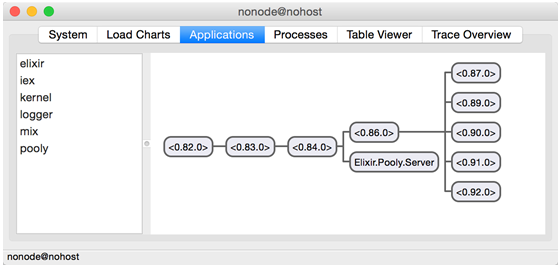
\includegraphics[width=0.8\linewidth]{6_4a.png}
    \caption{从 Observer 看到的 Pooly 的版本 1}
    \label{fig:6_4a}
\end{figure}


让我们开始杀死一个
worker。(我希望你没有大声朗读这本书)。你可以通过右键点击一个 worker
进程并选择 \emph{Kill process} 来做到这一点:

\begin{figure}[!ht]
    \centering
    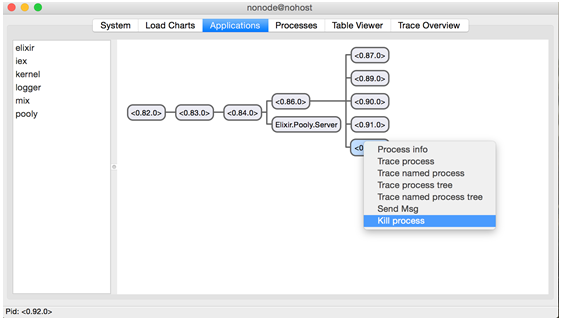
\includegraphics[width=0.8\linewidth]{6_5.png}
    \caption{从 Observer 杀死 worker}
    \label{fig:6_5}
\end{figure}

你会发现,监督器在被杀死的进程的位置生成了一个新的 worker。

更重要的是,单个 worker
的崩溃/退出并没有影响到监督树的其余部分。换句话说,那个单独的 worker
的崩溃只影响到\emph{那个} worker,而没有影响到其他任何东西。

\begin{figure}[!ht]
    \centering
    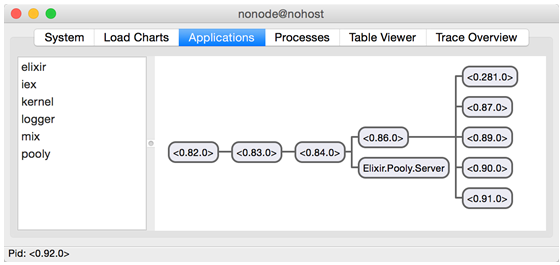
\includegraphics[width=0.8\linewidth]{6_6.png}
    \caption{监督器用新生成的 worker 替换了被杀死的 worker}
    \label{fig:6_6}
\end{figure}

现在,如果我们杀死 \texttt{Pooly.Server}
会发生什么呢?再次,右键点击 \texttt{Pooly.Server}
并选择 \emph{Kill process},就像这样:

\begin{figure}[!ht]
    \centering
    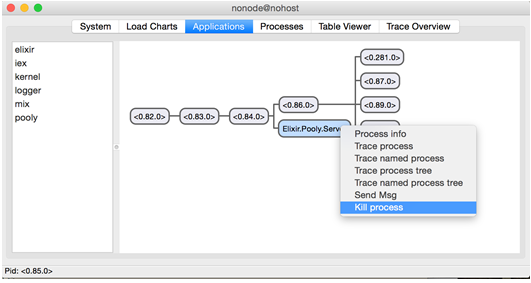
\includegraphics[width=0.8\linewidth]{6_7.png}
    \caption{从 Observer 杀死 Server 进程}
    \label{fig:6_7}
\end{figure}


这次,\emph{所有}的进程都被杀死,顶级监督器重新启动了\emph{所有}的子进程:

\begin{figure}[!ht]
    \centering
    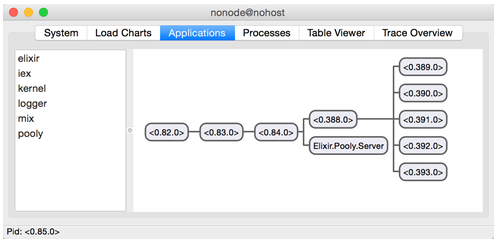
\includegraphics[width=0.8\linewidth]{6_8.png}
    \caption{杀死 Server 重新启动了顶级监督器下的所有进程}
    \label{fig:6_8}
\end{figure}


刚刚发生了什么?为什么杀死 \texttt{Pooly.Server}
会导致顶级监督器下的所有东西都死掉?仅仅是效果的描述就应该已经给出了一个重要的线索。顶级监督器的重启策略是什么?

让我们稍微回忆一下:

\begin{code}{}
\begin{minted}[linenos]{elixir}
defmodule Pooly.Supervisor do
  def init(pool_config) do
    # …
    opts = [strategy: :one_for_all]

    supervise(children, opts)
  end
end
\end{minted}
% \label{lst:id}
\end{code}

\texttt{:one\_for\_all} 重启策略完全解释了为什么杀死
\texttt{Pooly.Server}
会导致(并重新启动)其余的所有子进程。

 \section{练习}

\begin{enumerate}
\def\labelenumi{\arabic{enumi}.}
\item
  当你在 Observer 中杀死 \texttt{WorkerSupervisor}
  进程时会发生什么?你能解释发生了什么吗?
\item
  关闭和重启值。尝试使用各种关闭和重启值。例如,在
  \texttt{Pooly.WorkerSupervisor} 中,尝试将
  \texttt{opts} 从
\end{enumerate}

\begin{code}{}
\begin{minted}[linenos]{elixir}
opts = [strategy: :simple_one_for_one, max_restarts: 5, max_seconds: 5]
\end{minted}
% \label{lst:id}
\end{code}

改为类似于

\begin{code}{}
\begin{minted}[linenos]{elixir}
opts = [strategy: :simple_one_for_one, max_restarts: 0, max_seconds: 5]
\end{minted}
% \label{lst:id}
\end{code}

接下来,尝试将 \texttt{worker\_opts} 从

\begin{code}{}
\begin{minted}[linenos]{elixir}
worker_opts = [restart:  :permanent, function: f]
\end{minted}
% \label{lst:id}
\end{code}

改为

\begin{code}{}
\begin{minted}[linenos]{elixir}
worker_opts = [restart:  :temporary, function: f]
\end{minted}
% \label{lst:id}
\end{code}

记住要将 \texttt{opts} 设置回原始值。

 \section{总结}

在本章中,我们学习了:

\begin{itemize}

\item
  OTP Supervisor 行为
\item
  不同的监督器重启策略
\item
  使用 ETS 存储状态
\item
  如何构建监督器层次结构,包括静态和动态
\item
  各种监督器和子进程规范选项
\item
  实现一个非常基础的 worker 池应用程序
\end{itemize}

我们已经看到,通过使用不同的重启策略,监督器可以决定其子进程如何重启。更重要的是,再次依赖于重启策略,监督器能够将崩溃隔离到仅受影响的进程。

尽管 Pooly
的第一个版本很简单,但它让我们有机会尝试构建静态和动态的监督器层次结构。在前一种情况中,我们在
\texttt{Pooly.Supervisor} 的监督规范中声明
\texttt{Pooly.Server}
应该被监督。在后一种情况中,只有当
\texttt{Pooly.Server}
初始化时,\texttt{Pooly.WorkerSupervisor}
才会被添加到监督树中。

在接下来的章节中,我们将继续发展 Pooly
的设计,同时为其添加更多功能。同时,我们将探索 Supervisor 的更高级用法。

\protect\hyperlink{u7YNvHigi67GoJPRzPXBQf4}{****{[}1{]}****} 这是以 Mr.T的口气写的。
\protect\hyperlink{unZsK4dstzhrpK6CA9DbDs8}{****{[}2{]}****} 
\protect\hyperlink{u5UHZe9erUMjrZtCEGXEoxG}{****{[}3{]}****}
这在软件行业是很少见的。

/printnotes